\documentclass{standalone}
\usepackage{tikz}
\usetikzlibrary{patterns, positioning}

\begin{document}
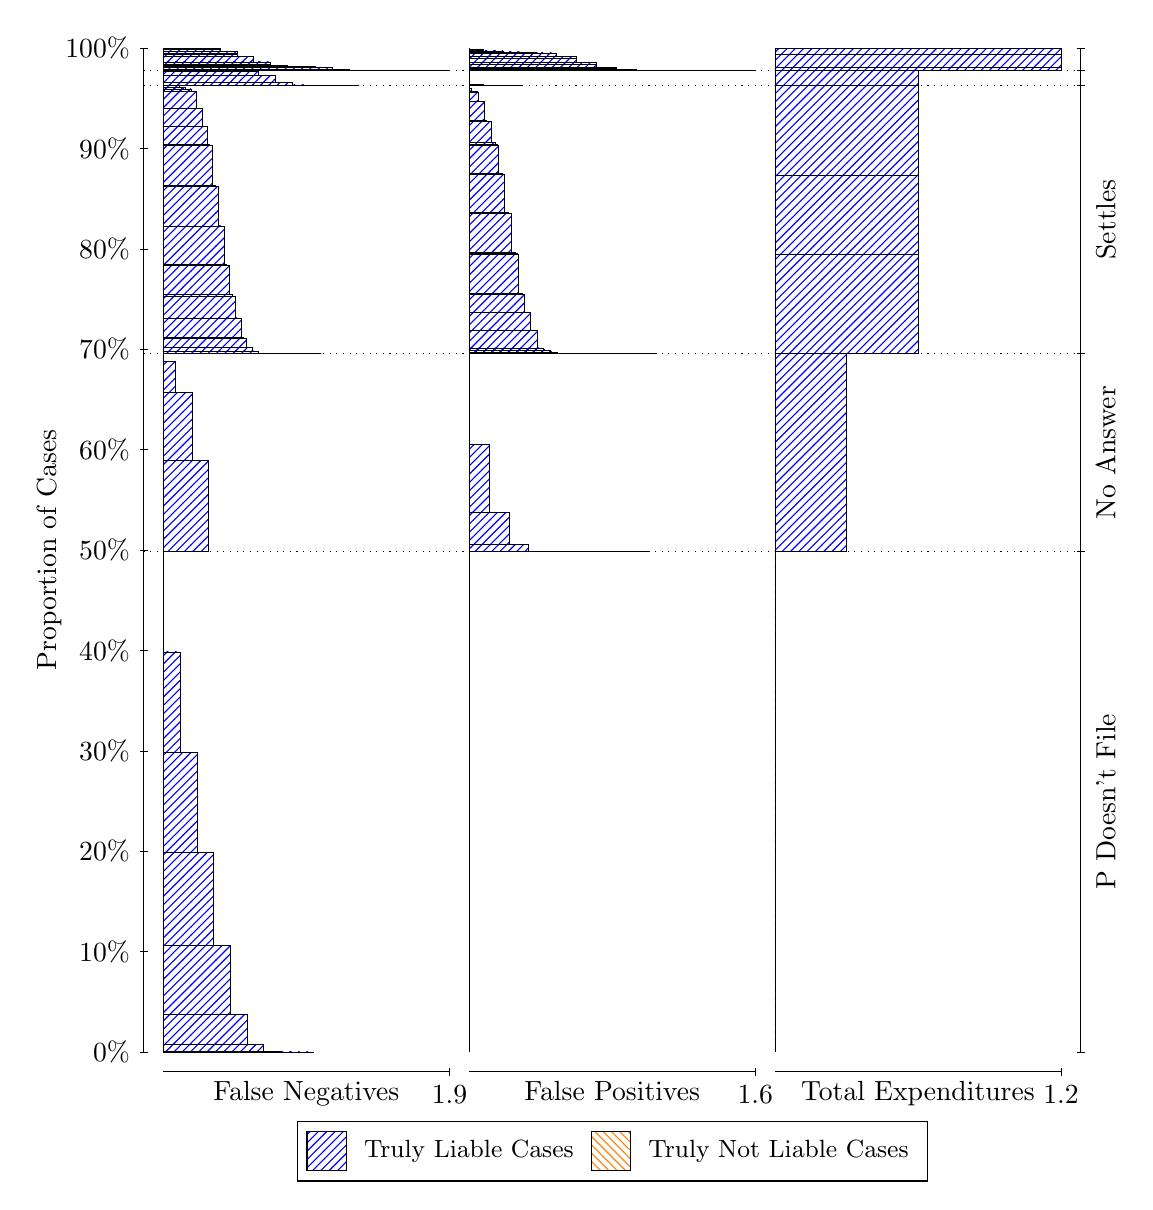
\begin{tikzpicture}
\draw[black, very thin] (1.5,1.75) -- (1.5,14.5);
\node[rotate=90, anchor=center] at (0.3, 8.125) {Proportion of Cases};
\draw[black, very thin] (1.45,1.75) -- (1.55,1.75);
\node[anchor=east] at (1.45, 1.75) {0\%};
\draw[black, very thin] (1.45,3.025) -- (1.55,3.025);
\node[anchor=east] at (1.45, 3.025) {10\%};
\draw[black, very thin] (1.45,4.3) -- (1.55,4.3);
\node[anchor=east] at (1.45, 4.3) {20\%};
\draw[black, very thin] (1.45,5.575) -- (1.55,5.575);
\node[anchor=east] at (1.45, 5.575) {30\%};
\draw[black, very thin] (1.45,6.85) -- (1.55,6.85);
\node[anchor=east] at (1.45, 6.85) {40\%};
\draw[black, very thin] (1.45,8.125) -- (1.55,8.125);
\node[anchor=east] at (1.45, 8.125) {50\%};
\draw[black, very thin] (1.45,9.4) -- (1.55,9.4);
\node[anchor=east] at (1.45, 9.4) {60\%};
\draw[black, very thin] (1.45,10.675) -- (1.55,10.675);
\node[anchor=east] at (1.45, 10.675) {70\%};
\draw[black, very thin] (1.45,11.95) -- (1.55,11.95);
\node[anchor=east] at (1.45, 11.95) {80\%};
\draw[black, very thin] (1.45,13.225) -- (1.55,13.225);
\node[anchor=east] at (1.45, 13.225) {90\%};
\draw[black, very thin] (1.45,14.5) -- (1.55,14.5);
\node[anchor=east] at (1.45, 14.5) {100\%};

\draw[black, very thin] (13.4,1.75) -- (13.4,14.5);
\draw[black, very thin] (13.35,1.75) -- (13.45,1.75);
\node[anchor=west] at (13.35, 1.75) {};
\draw[black, very thin] (13.35,8.1049) -- (13.45,8.1049);
\node[anchor=west] at (13.35, 8.1049) {};
\draw[black, very thin] (13.35,10.618) -- (13.45,10.618);
\node[anchor=west] at (13.35, 10.618) {};
\draw[black, very thin] (13.35,14.029) -- (13.45,14.029);
\node[anchor=west] at (13.35, 14.029) {};
\draw[black, very thin] (13.35,14.215) -- (13.45,14.215);
\node[anchor=west] at (13.35, 14.215) {};
\draw[black, very thin] (13.35,14.5) -- (13.45,14.5);
\node[anchor=west] at (13.35, 14.5) {};

\draw[black, very thin, pattern color=blue, pattern=north east lines] (1.75,1.75) rectangle (3.6623,1.75);
\draw[black, very thin, pattern color=blue, pattern=north east lines] (1.75,1.75) rectangle (3.4498,1.7503);
\draw[black, very thin, pattern color=blue, pattern=north east lines] (1.75,1.7503) rectangle (3.2373,1.7582);
\draw[black, very thin, pattern color=blue, pattern=north east lines] (1.75,1.7582) rectangle (3.0249,1.8421);
\draw[black, very thin, pattern color=blue, pattern=north east lines] (1.75,1.8421) rectangle (2.8124,2.2307);
\draw[black, very thin, pattern color=blue, pattern=north east lines] (1.75,2.2307) rectangle (2.5999,3.1046);
\draw[black, very thin, pattern color=blue, pattern=north east lines] (1.75,3.1046) rectangle (2.3874,4.2895);
\draw[black, very thin, pattern color=blue, pattern=north east lines] (1.75,4.2895) rectangle (2.175,5.5553);
\draw[black, very thin, pattern color=blue, pattern=north east lines] (1.75,5.5553) rectangle (1.9625,6.8299);
\draw[black, very thin, pattern color=orange, pattern=north west lines] (1.75,6.8299) rectangle (1.75,6.8299);
\draw[black, very thin, pattern color=blue, pattern=north east lines] (1.75,6.8299) rectangle (1.75,8.1049);
\draw[black, very thin, pattern color=blue, pattern=north east lines] (1.75,8.1049) rectangle (2.3237,9.26);
\draw[black, very thin, pattern color=blue, pattern=north east lines] (1.75,9.26) rectangle (2.1112,10.123);
\draw[black, very thin, pattern color=blue, pattern=north east lines] (1.75,10.123) rectangle (1.8987,10.523);
\draw[black, very thin, pattern color=orange, pattern=north west lines] (1.75,10.523) rectangle (1.75,10.523);
\draw[black, very thin, pattern color=blue, pattern=north east lines] (1.75,10.523) rectangle (1.75,10.618);
\draw[black, very thin, pattern color=blue, pattern=north east lines] (1.75,10.618) rectangle (3.7579,10.618);
\draw[black, very thin, pattern color=blue, pattern=north east lines] (1.75,10.618) rectangle (3.6623,10.618);
\draw[black, very thin, pattern color=blue, pattern=north east lines] (1.75,10.618) rectangle (3.5667,10.618);
\draw[black, very thin, pattern color=blue, pattern=north east lines] (1.75,10.618) rectangle (3.5454,10.618);
\draw[black, very thin, pattern color=blue, pattern=north east lines] (1.75,10.618) rectangle (3.4711,10.618);
\draw[black, very thin, pattern color=blue, pattern=north east lines] (1.75,10.618) rectangle (3.4498,10.618);
\draw[black, very thin, pattern color=blue, pattern=north east lines] (1.75,10.618) rectangle (3.3754,10.618);
\draw[black, very thin, pattern color=blue, pattern=north east lines] (1.75,10.618) rectangle (3.3542,10.618);
\draw[black, very thin, pattern color=blue, pattern=north east lines] (1.75,10.618) rectangle (3.3329,10.618);
\draw[black, very thin, pattern color=blue, pattern=north east lines] (1.75,10.618) rectangle (3.2798,10.618);
\draw[black, very thin, pattern color=blue, pattern=north east lines] (1.75,10.618) rectangle (3.2586,10.618);
\draw[black, very thin, pattern color=blue, pattern=north east lines] (1.75,10.618) rectangle (3.2373,10.618);
\draw[black, very thin, pattern color=blue, pattern=north east lines] (1.75,10.618) rectangle (3.1842,10.618);
\draw[black, very thin, pattern color=blue, pattern=north east lines] (1.75,10.618) rectangle (3.163,10.619);
\draw[black, very thin, pattern color=blue, pattern=north east lines] (1.75,10.619) rectangle (3.1417,10.619);
\draw[black, very thin, pattern color=blue, pattern=north east lines] (1.75,10.619) rectangle (3.1205,10.619);
\draw[black, very thin, pattern color=blue, pattern=north east lines] (1.75,10.619) rectangle (3.0886,10.622);
\draw[black, very thin, pattern color=blue, pattern=north east lines] (1.75,10.622) rectangle (3.0673,10.622);
\draw[black, very thin, pattern color=blue, pattern=north east lines] (1.75,10.622) rectangle (3.0461,10.622);
\draw[black, very thin, pattern color=blue, pattern=north east lines] (1.75,10.622) rectangle (3.0249,10.622);
\draw[black, very thin, pattern color=blue, pattern=north east lines] (1.75,10.622) rectangle (2.9717,10.622);
\draw[black, very thin, pattern color=blue, pattern=north east lines] (1.75,10.622) rectangle (2.9505,10.652);
\draw[black, very thin, pattern color=blue, pattern=north east lines] (1.75,10.652) rectangle (2.9292,10.652);
\draw[black, very thin, pattern color=blue, pattern=north east lines] (1.75,10.652) rectangle (2.908,10.653);
\draw[black, very thin, pattern color=blue, pattern=north east lines] (1.75,10.653) rectangle (2.8761,10.694);
\draw[black, very thin, pattern color=blue, pattern=north east lines] (1.75,10.694) rectangle (2.8549,10.694);
\draw[black, very thin, pattern color=blue, pattern=north east lines] (1.75,10.694) rectangle (2.8336,10.703);
\draw[black, very thin, pattern color=blue, pattern=north east lines] (1.75,10.703) rectangle (2.8124,10.703);
\draw[black, very thin, pattern color=blue, pattern=north east lines] (1.75,10.703) rectangle (2.8018,10.82);
\draw[black, very thin, pattern color=blue, pattern=north east lines] (1.75,10.82) rectangle (2.7593,10.824);
\draw[black, very thin, pattern color=blue, pattern=north east lines] (1.75,10.824) rectangle (2.738,11.069);
\draw[black, very thin, pattern color=blue, pattern=north east lines] (1.75,11.069) rectangle (2.7168,11.073);
\draw[black, very thin, pattern color=blue, pattern=north east lines] (1.75,11.073) rectangle (2.6955,11.074);
\draw[black, very thin, pattern color=blue, pattern=north east lines] (1.75,11.074) rectangle (2.6636,11.348);
\draw[black, very thin, pattern color=blue, pattern=north east lines] (1.75,11.348) rectangle (2.6424,11.349);
\draw[black, very thin, pattern color=blue, pattern=north east lines] (1.75,11.349) rectangle (2.6212,11.375);
\draw[black, very thin, pattern color=blue, pattern=north east lines] (1.75,11.375) rectangle (2.5999,11.376);
\draw[black, very thin, pattern color=blue, pattern=north east lines] (1.75,11.376) rectangle (2.5893,11.737);
\draw[black, very thin, pattern color=blue, pattern=north east lines] (1.75,11.737) rectangle (2.5468,11.754);
\draw[black, very thin, pattern color=blue, pattern=north east lines] (1.75,11.754) rectangle (2.5255,12.231);
\draw[black, very thin, pattern color=blue, pattern=north east lines] (1.75,12.231) rectangle (2.5043,12.239);
\draw[black, very thin, pattern color=blue, pattern=north east lines] (1.75,12.239) rectangle (2.483,12.241);
\draw[black, very thin, pattern color=blue, pattern=north east lines] (1.75,12.241) rectangle (2.4512,12.741);
\draw[black, very thin, pattern color=blue, pattern=north east lines] (1.75,12.741) rectangle (2.4299,12.742);
\draw[black, very thin, pattern color=blue, pattern=north east lines] (1.75,12.742) rectangle (2.4087,12.759);
\draw[black, very thin, pattern color=blue, pattern=north east lines] (1.75,12.759) rectangle (2.3874,12.76);
\draw[black, very thin, pattern color=blue, pattern=north east lines] (1.75,12.76) rectangle (2.3768,13.264);
\draw[black, very thin, pattern color=blue, pattern=north east lines] (1.75,13.264) rectangle (2.3343,13.276);
\draw[black, very thin, pattern color=blue, pattern=north east lines] (1.75,13.276) rectangle (2.3131,13.501);
\draw[black, very thin, pattern color=blue, pattern=north east lines] (1.75,13.501) rectangle (2.2918,13.504);
\draw[black, very thin, pattern color=blue, pattern=north east lines] (1.75,13.504) rectangle (2.2706,13.504);
\draw[black, very thin, pattern color=blue, pattern=north east lines] (1.75,13.504) rectangle (2.2387,13.734);
\draw[black, very thin, pattern color=blue, pattern=north east lines] (1.75,13.734) rectangle (2.2174,13.734);
\draw[black, very thin, pattern color=blue, pattern=north east lines] (1.75,13.734) rectangle (2.1962,13.736);
\draw[black, very thin, pattern color=blue, pattern=north east lines] (1.75,13.736) rectangle (2.175,13.737);
\draw[black, very thin, pattern color=blue, pattern=north east lines] (1.75,13.737) rectangle (2.1643,13.955);
\draw[black, very thin, pattern color=blue, pattern=north east lines] (1.75,13.955) rectangle (2.1218,13.957);
\draw[black, very thin, pattern color=blue, pattern=north east lines] (1.75,13.957) rectangle (2.1006,13.981);
\draw[black, very thin, pattern color=blue, pattern=north east lines] (1.75,13.981) rectangle (2.0793,13.981);
\draw[black, very thin, pattern color=blue, pattern=north east lines] (1.75,13.981) rectangle (2.0581,13.981);
\draw[black, very thin, pattern color=blue, pattern=north east lines] (1.75,13.981) rectangle (2.0262,14.005);
\draw[black, very thin, pattern color=blue, pattern=north east lines] (1.75,14.005) rectangle (2.005,14.005);
\draw[black, very thin, pattern color=blue, pattern=north east lines] (1.75,14.005) rectangle (1.9837,14.005);
\draw[black, very thin, pattern color=blue, pattern=north east lines] (1.75,14.005) rectangle (1.9625,14.005);
\draw[black, very thin, pattern color=blue, pattern=north east lines] (1.75,14.005) rectangle (1.9519,14.027);
\draw[black, very thin, pattern color=blue, pattern=north east lines] (1.75,14.027) rectangle (1.9094,14.027);
\draw[black, very thin, pattern color=blue, pattern=north east lines] (1.75,14.027) rectangle (1.8881,14.028);
\draw[black, very thin, pattern color=blue, pattern=north east lines] (1.75,14.028) rectangle (1.8669,14.028);
\draw[black, very thin, pattern color=blue, pattern=north east lines] (1.75,14.028) rectangle (1.8456,14.028);
\draw[black, very thin, pattern color=blue, pattern=north east lines] (1.75,14.028) rectangle (1.8137,14.028);
\draw[black, very thin, pattern color=blue, pattern=north east lines] (1.75,14.028) rectangle (1.7925,14.028);
\draw[black, very thin, pattern color=blue, pattern=north east lines] (1.75,14.028) rectangle (1.7712,14.028);
\draw[black, very thin, pattern color=orange, pattern=north west lines] (1.75,14.028) rectangle (1.75,14.028);
\draw[black, very thin, pattern color=blue, pattern=north east lines] (1.75,14.028) rectangle (1.75,14.029);
\draw[black, very thin, pattern color=blue, pattern=north east lines] (1.75,14.029) rectangle (4.236,14.029);
\draw[black, very thin, pattern color=blue, pattern=north east lines] (1.75,14.029) rectangle (4.0235,14.029);
\draw[black, very thin, pattern color=blue, pattern=north east lines] (1.75,14.029) rectangle (3.811,14.029);
\draw[black, very thin, pattern color=blue, pattern=north east lines] (1.75,14.029) rectangle (3.5985,14.031);
\draw[black, very thin, pattern color=blue, pattern=north east lines] (1.75,14.031) rectangle (3.3861,14.062);
\draw[black, very thin, pattern color=blue, pattern=north east lines] (1.75,14.062) rectangle (3.1736,14.154);
\draw[black, very thin, pattern color=blue, pattern=north east lines] (1.75,14.154) rectangle (2.9611,14.207);
\draw[black, very thin, pattern color=blue, pattern=north east lines] (1.75,14.207) rectangle (2.7486,14.214);
\draw[black, very thin, pattern color=blue, pattern=north east lines] (1.75,14.214) rectangle (2.5362,14.215);
\draw[black, very thin, pattern color=blue, pattern=north east lines] (1.75,14.215) rectangle (2.3237,14.215);
\draw[black, very thin, pattern color=orange, pattern=north west lines] (1.75,14.215) rectangle (1.75,14.215);
\draw[black, very thin, pattern color=blue, pattern=north east lines] (1.75,14.215) rectangle (5.3833,14.215);
\draw[black, very thin, pattern color=blue, pattern=north east lines] (1.75,14.215) rectangle (5.1709,14.215);
\draw[black, very thin, pattern color=blue, pattern=north east lines] (1.75,14.215) rectangle (4.9584,14.215);
\draw[black, very thin, pattern color=blue, pattern=north east lines] (1.75,14.215) rectangle (4.7459,14.215);
\draw[black, very thin, pattern color=blue, pattern=north east lines] (1.75,14.215) rectangle (4.7459,14.215);
\draw[black, very thin, pattern color=blue, pattern=north east lines] (1.75,14.215) rectangle (4.5334,14.215);
\draw[black, very thin, pattern color=blue, pattern=north east lines] (1.75,14.215) rectangle (4.5334,14.215);
\draw[black, very thin, pattern color=blue, pattern=north east lines] (1.75,14.215) rectangle (4.3847,14.215);
\draw[black, very thin, pattern color=blue, pattern=north east lines] (1.75,14.215) rectangle (4.321,14.216);
\draw[black, very thin, pattern color=blue, pattern=north east lines] (1.75,14.216) rectangle (4.321,14.217);
\draw[black, very thin, pattern color=blue, pattern=north east lines] (1.75,14.217) rectangle (4.1722,14.217);
\draw[black, very thin, pattern color=blue, pattern=north east lines] (1.75,14.217) rectangle (4.1085,14.227);
\draw[black, very thin, pattern color=blue, pattern=north east lines] (1.75,14.227) rectangle (4.1085,14.228);
\draw[black, very thin, pattern color=blue, pattern=north east lines] (1.75,14.228) rectangle (3.9597,14.228);
\draw[black, very thin, pattern color=blue, pattern=north east lines] (1.75,14.228) rectangle (3.896,14.25);
\draw[black, very thin, pattern color=blue, pattern=north east lines] (1.75,14.25) rectangle (3.896,14.25);
\draw[black, very thin, pattern color=blue, pattern=north east lines] (1.75,14.25) rectangle (3.7473,14.25);
\draw[black, very thin, pattern color=blue, pattern=north east lines] (1.75,14.25) rectangle (3.7473,14.25);
\draw[black, very thin, pattern color=blue, pattern=north east lines] (1.75,14.25) rectangle (3.6835,14.265);
\draw[black, very thin, pattern color=blue, pattern=north east lines] (1.75,14.265) rectangle (3.5348,14.265);
\draw[black, very thin, pattern color=blue, pattern=north east lines] (1.75,14.265) rectangle (3.5348,14.265);
\draw[black, very thin, pattern color=blue, pattern=north east lines] (1.75,14.265) rectangle (3.4711,14.267);
\draw[black, very thin, pattern color=blue, pattern=north east lines] (1.75,14.267) rectangle (3.3223,14.277);
\draw[black, very thin, pattern color=blue, pattern=north east lines] (1.75,14.277) rectangle (3.2586,14.277);
\draw[black, very thin, pattern color=blue, pattern=north east lines] (1.75,14.277) rectangle (3.2586,14.277);
\draw[black, very thin, pattern color=blue, pattern=north east lines] (1.75,14.277) rectangle (3.1098,14.295);
\draw[black, very thin, pattern color=blue, pattern=north east lines] (1.75,14.295) rectangle (3.1098,14.324);
\draw[black, very thin, pattern color=blue, pattern=north east lines] (1.75,14.324) rectangle (3.0461,14.324);
\draw[black, very thin, pattern color=blue, pattern=north east lines] (1.75,14.324) rectangle (3.0461,14.324);
\draw[black, very thin, pattern color=blue, pattern=north east lines] (1.75,14.324) rectangle (2.8974,14.398);
\draw[black, very thin, pattern color=blue, pattern=north east lines] (1.75,14.398) rectangle (2.8336,14.398);
\draw[black, very thin, pattern color=blue, pattern=north east lines] (1.75,14.398) rectangle (2.6849,14.426);
\draw[black, very thin, pattern color=blue, pattern=north east lines] (1.75,14.426) rectangle (2.6849,14.427);
\draw[black, very thin, pattern color=blue, pattern=north east lines] (1.75,14.427) rectangle (2.6849,14.459);
\draw[black, very thin, pattern color=blue, pattern=north east lines] (1.75,14.459) rectangle (2.6212,14.459);
\draw[black, very thin, pattern color=blue, pattern=north east lines] (1.75,14.459) rectangle (2.4724,14.49);
\draw[black, very thin, pattern color=blue, pattern=north east lines] (1.75,14.49) rectangle (2.4724,14.491);
\draw[black, very thin, pattern color=blue, pattern=north east lines] (1.75,14.491) rectangle (2.2599,14.493);
\draw[black, very thin, pattern color=blue, pattern=north east lines] (1.75,14.493) rectangle (2.2599,14.494);
\draw[black, very thin, pattern color=blue, pattern=north east lines] (1.75,14.494) rectangle (2.2599,14.499);
\draw[black, very thin, pattern color=blue, pattern=north east lines] (1.75,14.499) rectangle (2.0475,14.5);
\draw[black, very thin, pattern color=blue, pattern=north east lines] (1.75,14.5) rectangle (2.0475,14.5);
\draw[black, very thin, pattern color=blue, pattern=north east lines] (1.75,14.5) rectangle (1.835,14.5);
\draw[black, very thin, pattern color=blue, pattern=north east lines] (1.75,14.5) rectangle (1.835,14.5);
\draw[black, very thin, pattern color=orange, pattern=north west lines] (1.75,14.5) rectangle (1.75,14.5);
\draw[black, very thin, pattern color=blue, pattern=north east lines] (1.75,14.5) rectangle (1.75,14.5);
\draw[black, very thin, pattern color=orange, pattern=north west lines] (5.6333,1.75) rectangle (5.6333,1.75);
\draw[black, very thin, pattern color=blue, pattern=north east lines] (5.6333,1.75) rectangle (5.6333,8.1049);
\draw[black, very thin, pattern color=orange, pattern=north west lines] (5.6333,8.1049) rectangle (7.9042,8.1049);
\draw[black, very thin, pattern color=blue, pattern=north east lines] (5.6333,8.1049) rectangle (7.9042,8.1049);
\draw[black, very thin, pattern color=blue, pattern=north east lines] (5.6333,8.1049) rectangle (7.6519,8.1049);
\draw[black, very thin, pattern color=blue, pattern=north east lines] (5.6333,8.1049) rectangle (7.3995,8.1049);
\draw[black, very thin, pattern color=blue, pattern=north east lines] (5.6333,8.1049) rectangle (7.1472,8.1049);
\draw[black, very thin, pattern color=blue, pattern=north east lines] (5.6333,8.1049) rectangle (6.8949,8.105);
\draw[black, very thin, pattern color=blue, pattern=north east lines] (5.6333,8.105) rectangle (6.6426,8.1121);
\draw[black, very thin, pattern color=blue, pattern=north east lines] (5.6333,8.1121) rectangle (6.3903,8.2);
\draw[black, very thin, pattern color=blue, pattern=north east lines] (5.6333,8.2) rectangle (6.138,8.6);
\draw[black, very thin, pattern color=blue, pattern=north east lines] (5.6333,8.6) rectangle (5.8856,9.4631);
\draw[black, very thin, pattern color=blue, pattern=north east lines] (5.6333,9.4631) rectangle (5.6333,10.618);
\draw[black, very thin, pattern color=orange, pattern=north west lines] (5.6333,10.618) rectangle (8.0177,10.618);
\draw[black, very thin, pattern color=blue, pattern=north east lines] (5.6333,10.618) rectangle (8.0177,10.618);
\draw[black, very thin, pattern color=blue, pattern=north east lines] (5.6333,10.618) rectangle (7.7654,10.618);
\draw[black, very thin, pattern color=orange, pattern=north west lines] (5.6333,10.618) rectangle (7.6771,10.618);
\draw[black, very thin, pattern color=blue, pattern=north east lines] (5.6333,10.618) rectangle (7.6771,10.618);
\draw[black, very thin, pattern color=orange, pattern=north west lines] (5.6333,10.618) rectangle (7.5635,10.618);
\draw[black, very thin, pattern color=blue, pattern=north east lines] (5.6333,10.618) rectangle (7.5635,10.618);
\draw[black, very thin, pattern color=blue, pattern=north east lines] (5.6333,10.618) rectangle (7.5131,10.618);
\draw[black, very thin, pattern color=orange, pattern=north west lines] (5.6333,10.618) rectangle (7.45,10.618);
\draw[black, very thin, pattern color=blue, pattern=north east lines] (5.6333,10.618) rectangle (7.45,10.618);
\draw[black, very thin, pattern color=blue, pattern=north east lines] (5.6333,10.618) rectangle (7.4248,10.618);
\draw[black, very thin, pattern color=orange, pattern=north west lines] (5.6333,10.618) rectangle (7.3365,10.618);
\draw[black, very thin, pattern color=blue, pattern=north east lines] (5.6333,10.618) rectangle (7.3365,10.618);
\draw[black, very thin, pattern color=blue, pattern=north east lines] (5.6333,10.618) rectangle (7.3112,10.618);
\draw[black, very thin, pattern color=blue, pattern=north east lines] (5.6333,10.618) rectangle (7.2608,10.618);
\draw[black, very thin, pattern color=orange, pattern=north west lines] (5.6333,10.618) rectangle (7.2229,10.618);
\draw[black, very thin, pattern color=blue, pattern=north east lines] (5.6333,10.618) rectangle (7.2229,10.618);
\draw[black, very thin, pattern color=blue, pattern=north east lines] (5.6333,10.618) rectangle (7.1977,10.618);
\draw[black, very thin, pattern color=blue, pattern=north east lines] (5.6333,10.618) rectangle (7.1725,10.618);
\draw[black, very thin, pattern color=orange, pattern=north west lines] (5.6333,10.618) rectangle (7.1094,10.618);
\draw[black, very thin, pattern color=blue, pattern=north east lines] (5.6333,10.618) rectangle (7.1094,10.618);
\draw[black, very thin, pattern color=blue, pattern=north east lines] (5.6333,10.618) rectangle (7.0841,10.618);
\draw[black, very thin, pattern color=blue, pattern=north east lines] (5.6333,10.618) rectangle (7.0589,10.618);
\draw[black, very thin, pattern color=blue, pattern=north east lines] (5.6333,10.618) rectangle (7.0084,10.619);
\draw[black, very thin, pattern color=orange, pattern=north west lines] (5.6333,10.619) rectangle (6.9958,10.619);
\draw[black, very thin, pattern color=blue, pattern=north east lines] (5.6333,10.619) rectangle (6.9958,10.619);
\draw[black, very thin, pattern color=blue, pattern=north east lines] (5.6333,10.619) rectangle (6.9706,10.619);
\draw[black, very thin, pattern color=blue, pattern=north east lines] (5.6333,10.619) rectangle (6.9454,10.619);
\draw[black, very thin, pattern color=blue, pattern=north east lines] (5.6333,10.619) rectangle (6.9201,10.619);
\draw[black, very thin, pattern color=orange, pattern=north west lines] (5.6333,10.619) rectangle (6.8823,10.619);
\draw[black, very thin, pattern color=blue, pattern=north east lines] (5.6333,10.619) rectangle (6.8823,10.619);
\draw[black, very thin, pattern color=blue, pattern=north east lines] (5.6333,10.619) rectangle (6.8571,10.619);
\draw[black, very thin, pattern color=blue, pattern=north east lines] (5.6333,10.619) rectangle (6.8318,10.62);
\draw[black, very thin, pattern color=blue, pattern=north east lines] (5.6333,10.62) rectangle (6.8066,10.62);
\draw[black, very thin, pattern color=blue, pattern=north east lines] (5.6333,10.62) rectangle (6.7561,10.642);
\draw[black, very thin, pattern color=blue, pattern=north east lines] (5.6333,10.642) rectangle (6.7435,10.642);
\draw[black, very thin, pattern color=blue, pattern=north east lines] (5.6333,10.642) rectangle (6.7183,10.642);
\draw[black, very thin, pattern color=blue, pattern=north east lines] (5.6333,10.642) rectangle (6.6931,10.642);
\draw[black, very thin, pattern color=blue, pattern=north east lines] (5.6333,10.642) rectangle (6.6678,10.666);
\draw[black, very thin, pattern color=blue, pattern=north east lines] (5.6333,10.666) rectangle (6.63,10.666);
\draw[black, very thin, pattern color=blue, pattern=north east lines] (5.6333,10.666) rectangle (6.6047,10.667);
\draw[black, very thin, pattern color=blue, pattern=north east lines] (5.6333,10.667) rectangle (6.5795,10.69);
\draw[black, very thin, pattern color=blue, pattern=north east lines] (5.6333,10.69) rectangle (6.5543,10.692);
\draw[black, very thin, pattern color=blue, pattern=north east lines] (5.6333,10.692) rectangle (6.5038,10.911);
\draw[black, very thin, pattern color=blue, pattern=north east lines] (5.6333,10.911) rectangle (6.4912,10.911);
\draw[black, very thin, pattern color=blue, pattern=north east lines] (5.6333,10.911) rectangle (6.466,10.913);
\draw[black, very thin, pattern color=blue, pattern=north east lines] (5.6333,10.913) rectangle (6.4407,10.913);
\draw[black, very thin, pattern color=blue, pattern=north east lines] (5.6333,10.913) rectangle (6.4155,11.143);
\draw[black, very thin, pattern color=blue, pattern=north east lines] (5.6333,11.143) rectangle (6.3777,11.143);
\draw[black, very thin, pattern color=blue, pattern=north east lines] (5.6333,11.143) rectangle (6.3524,11.146);
\draw[black, very thin, pattern color=blue, pattern=north east lines] (5.6333,11.146) rectangle (6.3272,11.371);
\draw[black, very thin, pattern color=blue, pattern=north east lines] (5.6333,11.371) rectangle (6.302,11.384);
\draw[black, very thin, pattern color=blue, pattern=north east lines] (5.6333,11.384) rectangle (6.2515,11.887);
\draw[black, very thin, pattern color=blue, pattern=north east lines] (5.6333,11.887) rectangle (6.2389,11.889);
\draw[black, very thin, pattern color=blue, pattern=north east lines] (5.6333,11.889) rectangle (6.2137,11.905);
\draw[black, very thin, pattern color=blue, pattern=north east lines] (5.6333,11.905) rectangle (6.1884,11.907);
\draw[black, very thin, pattern color=blue, pattern=north east lines] (5.6333,11.907) rectangle (6.1632,12.406);
\draw[black, very thin, pattern color=blue, pattern=north east lines] (5.6333,12.406) rectangle (6.1253,12.408);
\draw[black, very thin, pattern color=blue, pattern=north east lines] (5.6333,12.408) rectangle (6.1001,12.416);
\draw[black, very thin, pattern color=blue, pattern=north east lines] (5.6333,12.416) rectangle (6.0749,12.893);
\draw[black, very thin, pattern color=blue, pattern=north east lines] (5.6333,12.893) rectangle (6.0497,12.91);
\draw[black, very thin, pattern color=blue, pattern=north east lines] (5.6333,12.91) rectangle (5.9992,13.271);
\draw[black, very thin, pattern color=blue, pattern=north east lines] (5.6333,13.271) rectangle (5.9866,13.272);
\draw[black, very thin, pattern color=blue, pattern=north east lines] (5.6333,13.272) rectangle (5.9613,13.298);
\draw[black, very thin, pattern color=blue, pattern=north east lines] (5.6333,13.298) rectangle (5.9361,13.299);
\draw[black, very thin, pattern color=blue, pattern=north east lines] (5.6333,13.299) rectangle (5.9109,13.573);
\draw[black, very thin, pattern color=blue, pattern=north east lines] (5.6333,13.573) rectangle (5.873,13.574);
\draw[black, very thin, pattern color=blue, pattern=north east lines] (5.6333,13.574) rectangle (5.8478,13.579);
\draw[black, very thin, pattern color=blue, pattern=north east lines] (5.6333,13.579) rectangle (5.8226,13.823);
\draw[black, very thin, pattern color=blue, pattern=north east lines] (5.6333,13.823) rectangle (5.7973,13.827);
\draw[black, very thin, pattern color=blue, pattern=north east lines] (5.6333,13.827) rectangle (5.7469,13.944);
\draw[black, very thin, pattern color=blue, pattern=north east lines] (5.6333,13.944) rectangle (5.7343,13.945);
\draw[black, very thin, pattern color=blue, pattern=north east lines] (5.6333,13.945) rectangle (5.709,13.953);
\draw[black, very thin, pattern color=blue, pattern=north east lines] (5.6333,13.953) rectangle (5.6838,13.953);
\draw[black, very thin, pattern color=blue, pattern=north east lines] (5.6333,13.953) rectangle (5.6586,13.995);
\draw[black, very thin, pattern color=blue, pattern=north east lines] (5.6333,13.995) rectangle (5.6333,14.029);
\draw[black, very thin, pattern color=orange, pattern=north west lines] (5.6333,14.029) rectangle (6.3146,14.029);
\draw[black, very thin, pattern color=blue, pattern=north east lines] (5.6333,14.029) rectangle (6.3146,14.029);
\draw[black, very thin, pattern color=blue, pattern=north east lines] (5.6333,14.029) rectangle (6.0623,14.029);
\draw[black, very thin, pattern color=blue, pattern=north east lines] (5.6333,14.029) rectangle (5.81,14.037);
\draw[black, very thin, pattern color=blue, pattern=north east lines] (5.6333,14.037) rectangle (5.6333,14.215);
\draw[black, very thin, pattern color=orange, pattern=north west lines] (5.6333,14.215) rectangle (9.2667,14.215);
\draw[black, very thin, pattern color=blue, pattern=north east lines] (5.6333,14.215) rectangle (9.2667,14.215);
\draw[black, very thin, pattern color=orange, pattern=north west lines] (5.6333,14.215) rectangle (9.0144,14.215);
\draw[black, very thin, pattern color=blue, pattern=north east lines] (5.6333,14.215) rectangle (9.0144,14.215);
\draw[black, very thin, pattern color=orange, pattern=north west lines] (5.6333,14.215) rectangle (8.762,14.215);
\draw[black, very thin, pattern color=blue, pattern=north east lines] (5.6333,14.215) rectangle (8.762,14.215);
\draw[black, very thin, pattern color=blue, pattern=north east lines] (5.6333,14.215) rectangle (8.5097,14.215);
\draw[black, very thin, pattern color=orange, pattern=north west lines] (5.6333,14.215) rectangle (8.5097,14.215);
\draw[black, very thin, pattern color=blue, pattern=north east lines] (5.6333,14.215) rectangle (8.5097,14.215);
\draw[black, very thin, pattern color=blue, pattern=north east lines] (5.6333,14.215) rectangle (8.2574,14.215);
\draw[black, very thin, pattern color=orange, pattern=north west lines] (5.6333,14.215) rectangle (8.2574,14.215);
\draw[black, very thin, pattern color=blue, pattern=north east lines] (5.6333,14.215) rectangle (8.2574,14.215);
\draw[black, very thin, pattern color=blue, pattern=north east lines] (5.6333,14.215) rectangle (8.0051,14.216);
\draw[black, very thin, pattern color=orange, pattern=north west lines] (5.6333,14.216) rectangle (8.0051,14.216);
\draw[black, very thin, pattern color=blue, pattern=north east lines] (5.6333,14.216) rectangle (8.0051,14.216);
\draw[black, very thin, pattern color=blue, pattern=north east lines] (5.6333,14.216) rectangle (7.7528,14.22);
\draw[black, very thin, pattern color=orange, pattern=north west lines] (5.6333,14.22) rectangle (7.7528,14.22);
\draw[black, very thin, pattern color=blue, pattern=north east lines] (5.6333,14.22) rectangle (7.7528,14.224);
\draw[black, very thin, pattern color=blue, pattern=north east lines] (5.6333,14.224) rectangle (7.7528,14.224);
\draw[black, very thin, pattern color=blue, pattern=north east lines] (5.6333,14.224) rectangle (7.7528,14.224);
\draw[black, very thin, pattern color=blue, pattern=north east lines] (5.6333,14.224) rectangle (7.5005,14.243);
\draw[black, very thin, pattern color=orange, pattern=north west lines] (5.6333,14.243) rectangle (7.5005,14.243);
\draw[black, very thin, pattern color=blue, pattern=north east lines] (5.6333,14.243) rectangle (7.5005,14.255);
\draw[black, very thin, pattern color=blue, pattern=north east lines] (5.6333,14.255) rectangle (7.5005,14.255);
\draw[black, very thin, pattern color=orange, pattern=north west lines] (5.6333,14.255) rectangle (7.3238,14.255);
\draw[black, very thin, pattern color=blue, pattern=north east lines] (5.6333,14.255) rectangle (7.3238,14.255);
\draw[black, very thin, pattern color=blue, pattern=north east lines] (5.6333,14.255) rectangle (7.2481,14.257);
\draw[black, very thin, pattern color=blue, pattern=north east lines] (5.6333,14.257) rectangle (7.2481,14.293);
\draw[black, very thin, pattern color=blue, pattern=north east lines] (5.6333,14.293) rectangle (7.2481,14.317);
\draw[black, very thin, pattern color=orange, pattern=north west lines] (5.6333,14.317) rectangle (7.0715,14.317);
\draw[black, very thin, pattern color=blue, pattern=north east lines] (5.6333,14.317) rectangle (7.0715,14.317);
\draw[black, very thin, pattern color=blue, pattern=north east lines] (5.6333,14.317) rectangle (6.9958,14.32);
\draw[black, very thin, pattern color=blue, pattern=north east lines] (5.6333,14.32) rectangle (6.9958,14.365);
\draw[black, very thin, pattern color=blue, pattern=north east lines] (5.6333,14.365) rectangle (6.9958,14.391);
\draw[black, very thin, pattern color=blue, pattern=north east lines] (5.6333,14.391) rectangle (6.8192,14.391);
\draw[black, very thin, pattern color=orange, pattern=north west lines] (5.6333,14.391) rectangle (6.8192,14.391);
\draw[black, very thin, pattern color=blue, pattern=north east lines] (5.6333,14.391) rectangle (6.8192,14.391);
\draw[black, very thin, pattern color=blue, pattern=north east lines] (5.6333,14.391) rectangle (6.7435,14.396);
\draw[black, very thin, pattern color=blue, pattern=north east lines] (5.6333,14.396) rectangle (6.7435,14.396);
\draw[black, very thin, pattern color=blue, pattern=north east lines] (5.6333,14.396) rectangle (6.7435,14.432);
\draw[black, very thin, pattern color=blue, pattern=north east lines] (5.6333,14.432) rectangle (6.7435,14.438);
\draw[black, very thin, pattern color=blue, pattern=north east lines] (5.6333,14.438) rectangle (6.5669,14.438);
\draw[black, very thin, pattern color=orange, pattern=north west lines] (5.6333,14.438) rectangle (6.5669,14.438);
\draw[black, very thin, pattern color=blue, pattern=north east lines] (5.6333,14.438) rectangle (6.5669,14.438);
\draw[black, very thin, pattern color=blue, pattern=north east lines] (5.6333,14.438) rectangle (6.5669,14.438);
\draw[black, very thin, pattern color=blue, pattern=north east lines] (5.6333,14.438) rectangle (6.4912,14.441);
\draw[black, very thin, pattern color=blue, pattern=north east lines] (5.6333,14.441) rectangle (6.4912,14.448);
\draw[black, very thin, pattern color=blue, pattern=north east lines] (5.6333,14.448) rectangle (6.3146,14.449);
\draw[black, very thin, pattern color=orange, pattern=north west lines] (5.6333,14.449) rectangle (6.3146,14.449);
\draw[black, very thin, pattern color=blue, pattern=north east lines] (5.6333,14.449) rectangle (6.3146,14.45);
\draw[black, very thin, pattern color=blue, pattern=north east lines] (5.6333,14.45) rectangle (6.3146,14.45);
\draw[black, very thin, pattern color=blue, pattern=north east lines] (5.6333,14.45) rectangle (6.2389,14.45);
\draw[black, very thin, pattern color=blue, pattern=north east lines] (5.6333,14.45) rectangle (6.2389,14.45);
\draw[black, very thin, pattern color=blue, pattern=north east lines] (5.6333,14.45) rectangle (6.2389,14.45);
\draw[black, very thin, pattern color=blue, pattern=north east lines] (5.6333,14.45) rectangle (6.0623,14.464);
\draw[black, very thin, pattern color=blue, pattern=north east lines] (5.6333,14.464) rectangle (6.0623,14.464);
\draw[black, very thin, pattern color=blue, pattern=north east lines] (5.6333,14.464) rectangle (5.9866,14.464);
\draw[black, very thin, pattern color=blue, pattern=north east lines] (5.6333,14.464) rectangle (5.9866,14.464);
\draw[black, very thin, pattern color=blue, pattern=north east lines] (5.6333,14.464) rectangle (5.81,14.476);
\draw[black, very thin, pattern color=blue, pattern=north east lines] (5.6333,14.476) rectangle (5.81,14.477);
\draw[black, very thin, pattern color=blue, pattern=north east lines] (5.6333,14.477) rectangle (5.81,14.487);
\draw[black, very thin, pattern color=blue, pattern=north east lines] (5.6333,14.487) rectangle (5.7343,14.487);
\draw[black, very thin, pattern color=blue, pattern=north east lines] (5.6333,14.487) rectangle (5.7343,14.487);
\draw[black, very thin, pattern color=blue, pattern=north east lines] (5.6333,14.487) rectangle (5.7343,14.487);
\draw[black, very thin, pattern color=blue, pattern=north east lines] (5.6333,14.487) rectangle (5.6333,14.5);
\draw[black, very thin, pattern color=orange, pattern=north west lines] (9.5167,1.75) rectangle (9.5167,1.75);
\draw[black, very thin, pattern color=blue, pattern=north east lines] (9.5167,1.75) rectangle (9.5167,8.1049);
\draw[black, very thin, pattern color=orange, pattern=north west lines] (9.5167,8.1049) rectangle (10.425,8.1049);
\draw[black, very thin, pattern color=blue, pattern=north east lines] (9.5167,8.1049) rectangle (10.425,10.618);
\draw[black, very thin, pattern color=orange, pattern=north west lines] (9.5167,10.618) rectangle (11.333,10.618);
\draw[black, very thin, pattern color=blue, pattern=north east lines] (9.5167,10.618) rectangle (11.333,11.883);
\draw[black, very thin, pattern color=orange, pattern=north west lines] (9.5167,11.883) rectangle (11.333,11.883);
\draw[black, very thin, pattern color=blue, pattern=north east lines] (9.5167,11.883) rectangle (11.333,12.887);
\draw[black, very thin, pattern color=orange, pattern=north west lines] (9.5167,12.887) rectangle (11.333,12.887);
\draw[black, very thin, pattern color=blue, pattern=north east lines] (9.5167,12.887) rectangle (11.333,14.029);
\draw[black, very thin, pattern color=orange, pattern=north west lines] (9.5167,14.029) rectangle (11.333,14.029);
\draw[black, very thin, pattern color=blue, pattern=north east lines] (9.5167,14.029) rectangle (11.333,14.215);
\draw[black, very thin, pattern color=orange, pattern=north west lines] (9.5167,14.215) rectangle (13.15,14.215);
\draw[black, very thin, pattern color=blue, pattern=north east lines] (9.5167,14.215) rectangle (13.15,14.259);
\draw[black, very thin, pattern color=orange, pattern=north west lines] (9.5167,14.259) rectangle (13.15,14.259);
\draw[black, very thin, pattern color=blue, pattern=north east lines] (9.5167,14.259) rectangle (13.15,14.419);
\draw[black, very thin, pattern color=orange, pattern=north west lines] (9.5167,14.419) rectangle (13.15,14.419);
\draw[black, very thin, pattern color=blue, pattern=north east lines] (9.5167,14.419) rectangle (13.15,14.5);
\draw[black, dotted] (1.5,8.1049) -- (13.4,8.1049);
\draw[black, dotted] (1.5,10.618) -- (13.4,10.618);
\draw[black, dotted] (1.5,14.029) -- (13.4,14.029);
\draw[black, dotted] (1.5,14.215) -- (13.4,14.215);
\draw[black, very thin] (1.75,1.5) -- (5.3833,1.5);
\node[anchor=north] at (3.5667, 1.5) {False Negatives};
\draw[black, very thin] (5.3833,1.45) -- (5.3833,1.55);
\node[anchor=north] at (5.3833, 1.45) {1.9};

\draw[black, very thin] (5.6333,1.5) -- (9.2667,1.5);
\node[anchor=north] at (7.45, 1.5) {False Positives};
\draw[black, very thin] (9.2667,1.45) -- (9.2667,1.55);
\node[anchor=north] at (9.2667, 1.45) {1.6};

\draw[black, very thin] (9.5167,1.5) -- (13.15,1.5);
\node[anchor=north] at (11.333, 1.5) {Total Expenditures};
\draw[black, very thin] (13.15,1.45) -- (13.15,1.55);
\node[anchor=north] at (13.15, 1.45) {1.2};

\node[black, centered, rotate=90] at (13.72, 4.9274) {P Doesn't File};
\node[black, centered, rotate=90] at (13.72, 9.3615) {No Answer};
\node[black, centered, rotate=90] at (13.72, 12.324) {Settles};



\draw (7.449999999999999,1.5) node[draw=none] (baseCoordinate) {};
\begin{scope}[align=center]
        \matrix[scale=0.5, draw=black, below=0.5cm of baseCoordinate, nodes={draw}, column sep=0.1cm]{
            \node[rectangle, draw, minimum width=0.5cm, minimum height=0.5cm, pattern=north east lines, pattern color=blue] {}; &
            \node[draw=none, font=\small] (B) {Truly Liable Cases}; &
            \node[rectangle, draw, minimum width=0.5cm, minimum height=0.5cm, pattern=north west lines, pattern color=orange] {}; &
            \node[draw=none, font=\small] (B) {Truly Not Liable Cases}; \\
            };
\end{scope}

\end{tikzpicture}
\end{document}